\documentclass[conference, 10pt, twocolumn]{ieeeconf}

\IEEEoverridecommandlockouts
\overrideIEEEmargins

\usepackage[usenames]{color}
\usepackage{enumerate}
\usepackage{url}
\usepackage{amsfonts,mathrsfs}
\usepackage{amssymb,amsmath}
\usepackage{verbatim}
\usepackage{acronym}
\usepackage{mathtools}
\usepackage{graphicx}
\usepackage{bbm}
\usepackage{float}
\usepackage{subfigure}

\DeclareGraphicsExtensions{.pdf,.jpeg,.png}



%\newcommand{\remove}[1]{}
%\def\jnt#1{{{\bf #1}}}
\def\rasoul#1{{\color{blue}#1}}
%\long\def\red#1{{{\color{red}#1}}}
\def\an#1{{{\bf \color{red}#1}}}
\def\fskip#1{}

\newcounter{note}
\newtheorem{theorem}{Theorem}
\newtheorem{assumption}{Assumption}
\newtheorem{algorithm}[theorem]{Algorithm}
\newtheorem{axiom}[theorem]{Axiom}
\newtheorem{case}[theorem]{Case}
\newtheorem{claim}[theorem]{Claim}
\newtheorem{conclusion}[theorem]{Conclusion}
\newtheorem{condition}[theorem]{Condition}
\newtheorem{conjecture}[theorem]{Conjecture}
\newtheorem{corollary}{Corollary}
\newtheorem{criterion}[theorem]{Criterion}
\newtheorem{definition}{Definition}
\newtheorem{example}{Example}
\newtheorem{exercise}[theorem]{Exercise}
\newtheorem{lemma}{Lemma}
\newtheorem{notation}[note]{Notation}
\newtheorem{problem}[theorem]{Problem}
\newtheorem{proposition}[theorem]{Proposition}
\newtheorem{remark}{Remark}
\newtheorem{solution}[theorem]{Solution}
\newtheorem{summary}[theorem]{Summary}
\newtheorem{acknowledgement}{Acknowledgement}


%\textwidth 6.2in \textheight 9in \setlength{\topmargin}{-0.3in}
%\setlength{\oddsidemargin}{0.1in} \setlength{\evensidemargin}{0.1in}
%\renewcommand{\theequation}{\thesection.\arabic{equation}}
\renewcommand{\theenumi}{\arabic{enumi}}
\newcommand{\qed}{\ \ {\bf q.e.d.}}

\def\1{{\bf 1}}
\def\al{\alpha}
\def\E{\mathcal{E}}
\def\Eb{\overline{\E}}
\def\L{\mathcal{L}}
\def\A{\mathcal{A}}
\def\Ps{P_{\sigma}}
\def\e{{\bf e}}
\def\ei{{\e^{(i)}}}
\def\ej{{\e^{(j)}}}
\def\ek{{\e^{(k)}}}
\def\B{{\mathcal B}}
\def\Pm{{\mathcal P}}
\def\Gb{\overline{G}}
\def\N{\mathbb{N}}
\def\F{\mathscr{F}}
\def\Finf{\mathscr{F}^{\infty}}


\def\ol{\bar}
\def\Rd{\mathbb{R}^d}
\def\l{\lambda}
\def\b{\beta}
\def\d{\delta}
\def\e{\epsilon}
\def\g{\gamma}
\def\a{\alpha}
\def\N{\mathcal{N}}
\def\s{\sigma}
\def\tl{\tilde}
\def\k{\kappa}
\def\o{\omega}
\def\rn{\mathbb{R}^n}

\def\R{\mathbb{R}}
\def\re{\mathbb{R}}
\def\gr{\nabla}
\def\cone{{\rm cone}}
\def\dist{{\rm dist}}
\def\t{\tau}
\def\qed{\ {\bf Q.E.D.}}
\def\S{\mathscr{S}}
\def\bS{\mathbb{S}}
\def\cS{\mathcal{S}}
\def\I{\mathscr{I}}
\def\Z{\mathbb{Z}}

\newcommand{\EXP}[1]{\mathsf{E}\!\left[#1\right] }
\newcommand{\prob}[1]{\mathsf{Pr}\left( #1 \right)}
\newcommand{\remove}[1]{}
\newcommand{\Rm}{\mathbb{R}^m}
\newcommand{\lra}{\leftrightarrow}
\newcommand{\lrA}{\Leftrightarrow}
\newcommand{\M}{\mathscr{M}_2}
\newcommand{\diag}{\mbox{diag}}
\newcommand{\Ginf}{G^{\infty}}
\newcommand{\Einf}{\mathscr{E}^{\inf}}
\newcommand{\tw}{\tilde{W}}
\newcommand{\xc}{\{x(k)\}}
\DeclarePairedDelimiter\ceil{\lceil}{\rceil}
\DeclarePairedDelimiter\floor{\lfloor}{\rfloor}

\newcommand{\todo}[1]{\vspace{5 mm}\par \noindent \marginpar{\textsc{ToDo}}
\framebox{\begin{minipage}[c]{0.9 \columnwidth} \tt #1
\end{minipage}}\vspace{5 mm}\par}

\def\argmin{\mathop{\rm argmin}}
\def\an #1{{\color{red} #1}}

\begin{document}
\title{Random Tree Search Algorithm for Nash Equilibrium in Capacitated Selfish
Replication Games}
\author{\authorblockN{Seyed Nematollah Ahmadyan\textdagger, Seyed Rasoul Etesami\textdaggerdbl, H. Vincent Poor\textdaggerdbl}
  \authorblockA{}
\thanks{\textdagger Seyed Nematollah Ahmadyan is with
Coordinated Science Laboratory,
Department of Electrical and Computer Engineering,
University of Illinois at Urbana-Champaign, Urbana, IL, 61801;
E-mail: {ahmadya2}@illinois.edu}
\thanks{
\textdaggerdbl Seyed Rasoul Etesami and H. Vincent Poor are with
Department of Electrical Engineering,
Princeton University, NJ, 08644;
E-mail: etesami,poor@Princeton.EDU}
}
\maketitle
\begin{abstract}
In this paper we consider a resource allocation
game with limited capacities over large scale networks and
propose a novel randomized algorithm for searching its purestrategy
Nash equilibrium points. It is known that such games
always admit a pure-strategy Nash equilibrium and benefit
from having a low price of anarchy. However, the best
theoretical results only provide a quasi-polynomial constant
approximation algorithm of the equilibrium points over general
networks. Here, we search the state space of the resource
allocation game for its equilibrium points. We use a random
tree based search methods to minimize a proper objective
function and direct the search toward the pure-strategy Nash
equilibrium points of the system. Through empirical results, we
demonstrate that in comparison to the best known theoretical
bounds, our technique is more efficient.
\end{abstract}
\begin{keywords}
Capacitated selfish replication game; pure Nash equilibrium (NE); Random tree search algorithm.
\end{keywords}

\section{Introduction}
With myriads of data from social science and emergence of large scale social and economic networks, studying the evolutionary behavior of complex decision systems has become a major issue in recent years. In fact, game theory is one of the strong mathematical tools which has proven quite useful in capturing and modeling the complex nature of human decision making in social and economics networks. Despite numerous advances and contributions made in this field of study, there are a lot of barriers and limitations concerning computational issues of different games such as finding Nash equilibrium points or even approximation the equilibrium points of the system.  
 

In this context, we consider in this paper a class of problems known as resource allocation problems. In general, resource allocation games are referred to a class of games in which a set of agents or players are competing for the same set of resources and has many applications in various areas such as load balancing, peer-to-peer systems, congestion games, web-caches, content management, and market sharing games among many others \cite{pollatos2008social,pacifici2012convergence,gopalakrishnan2012cache,goemans2006market,masucci2014strategic,ackermann2008impact,fabrikant2004complexity}. In fact, one of the important features of such games is to increase the reliability of the entire network with respect to customer needs and to improve the availability of the resources for users.            

Typically, resource allocations games can be divided in two general groups: \textit{uncapacitated} and \textit{capacitated}. In uncapacitated allocation games the agents can keep even up to all the possible resources in their caches. However, there is an associated cost of keeping certain resources in the catch and this eliminates the posibility that every agent keep all the available resources in its catch. An instance of such games has been studied in \cite{chun2004selfish}, where the authors were able to fully characterize the set of equilibrium points. However, in the capaciteted case the situation could be much more complicated as the constraints on the capacities of the agents couples the actions of agents much more than in the uncapacitated case. As a result there is no comparable characterization of equilibrium points in capacitated selfish replication games. 

In this paper we focus on an instance of capacitated resource allocation games with binary preferences as was introduced in \cite{gopalakrishnan2012cache}, where ``binary preferences" captures the behavioral pattern where players are equally interested in some objects. In the balance of this paper, our focus will be on such games, which for simplicity we refer to as CSR games. In fact, CSR games are defined in terms of a set of available resources for each player, where the players are allowed to communicate through an undirected communication graph. Such a communication graph identifies the access cost among the players, and the goal for each player is to satisfy his/her customers' needs with minimum cost. 

The problem of finding an equilibrium for CSR games have been studied in \cite{gopalakrishnan2012cache,etesami2014pure}. It was shown in \cite{gopalakrishnan2012cache} that when the number of resources is 2, there exists a polynomial time algorithm $\mathcal{O}(n^3)$ to find an equilibrium, where $n$ is the number of players in the game. This result has been improved in \cite{etesami2014pure} to a linear time algorithm $\mathcal{O}(n)$ when the number of resources is bounded above by 5. Moreover, a quasi-polynomial approximation algorithm $\mathcal{O}(n^{\ln D})$ for approximating any Nash equilibrium of the system within a constant factor has been given in \cite{etesami2015approximation}, where $D$ denotes the diameter of the network. In this paper we consider CSR games over general undirected networks and devise a randomized algorithm based on random tree search to find the Nash equilibrium points of the system.
 
The paper is organized as follows. In Section~\ref{sec:game-model}, we introduce CSR games over general undirected networks and review some relevant existing results on this problem. In Section \ref{sec:main-I}, we  characterize the equilibrium points of the system as maximizers of a well-defined function and theoretically justify that randomization can be quite beneficial for maximizing such function under certain cases. Following this, in Section \ref{sec:apx-alg} we device a random tree search algorithm for maximize the objective function. Through numerous simulation results we show that this method can be indeed quite effective. We conclude the paper with identifying future directions of research in Section~\ref{sec:conclusion}. 

\textbf{Notations}: 
For a positive integer $n$, we let $[n]:=\{1,2,\ldots,n\}$. We use $\mathcal{G}=([n], \mathcal{E})$ for an undirected underlying network with a node set $\{1,2,\ldots,n\}$ and an edge set $\mathcal{E}$. For any two nodes $i, j \in [n]$, we let $d_{\mathcal{G}}(i,j)$ be the graphical distance between them, that is, the length of a shortest path which connects $i$ and $j$. For an arbitrary node $i\in [n]$ and an integer $r\ge 0$, we define a ball of radius $r$ and center $i$ to be the set of all the nodes in the graph $\mathcal{G}$ whose graphical distance to the node $i$ is at most $r$, i.e., $B_{\mathcal{G}}(i,r)=\{x\in \mathcal{V}| d_{\mathcal{G}}(i,x)\leq r\}$. We denote the cardinality of a finite set $A$ by $|A|$.


\section{Problem Formulation and Existing Results}\label{sec:game-model}

In this section we first introduce the capacitated selfish replication game with binary preferences as was introduced in \cite{gopalakrishnan2012cache}. In the balance of this paper, our focus will be on such games, which for simplicity we refer to as CSR games.

\subsection{CSR Game Model}
We start with a set of $[n]=\{1,2,\ldots,n\}$ nodes (players) which are connected by an undirected graph $\mathcal{G}=([n], \mathcal{E})$. We denote the set of all resources by $O=\{o_1, o_2,\ldots, o_k\}$. For simplicity, but without much loss of generality, we assume that each node can hold only one resource in its cache. All the results can in fact be extended to CSR games with different capacities (see Remark \ref{rem:varying-cache} below). Moreover, we assume that each node has access to all the resources. For a particular allocation $P=(P_1, P_2, \ldots, P_n)$, we define the sum cost function $C_i(P)$ of the $i$th player as follows:
\begin{align}\label{eq:CSR-cost-formulation}
C_i(P)=\sum_{o\in O\setminus \{P_i\}}d_{\mathcal{G}}(i, \sigma_i(P,o)),
\end{align}
where $\sigma_i(P,o)$ is $i$'s nearest node holding $o$ in $P$. Given an allocation profile $P$ we define the {\bf\textit{radius}} of agent $i$, denoted by $r_i(P)$, to be the distance between node $i$ and the nearest node other than her holding the same resource as $i$, i.e., $r_i(P)=\min_{ j\neq i, P_j=P_i}d_{\mathcal{G}}(i,j)$. Note that if there does not exist such a node, we simply define $r_i(P)=D$, where $D$ is the diameter of the network. We suppress the dependence of $r_i(P)$ on $P$ whenever there is no ambiguity. In Figure \ref{fig:example-model} we have illustrated an instance of the CSR game for $n=11$ and $|O|=3$, and provided the associated costs and radii for two players $i=1,8$.

\begin{figure}[htb]
\vspace{-1.5cm}
\begin{center}
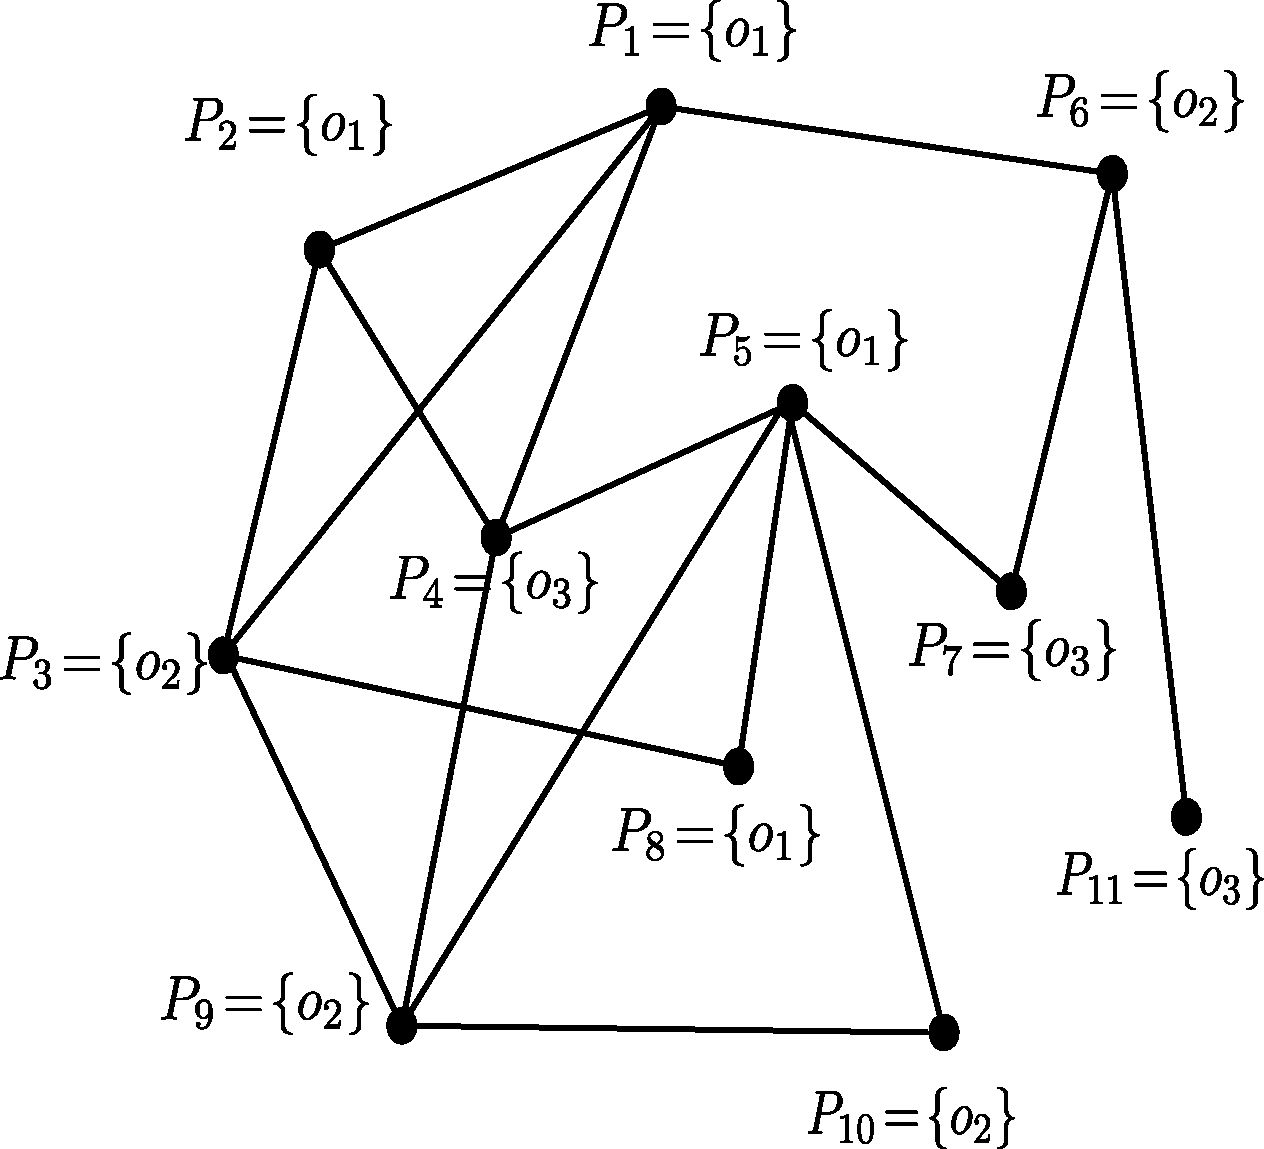
\includegraphics[totalheight=.22\textheight,
width=.4\textwidth,viewport=-50 0 800 750]{example} \hspace{0.4in}
\end{center}
\vspace{-0.3cm}\caption{CSR game with $n=11$ players and $O=\{o_1,o_2,o_3\}$ resources. We have $C_1(P)=0+1+1=2, C_8(P)=0+1+2=3$ and $r_1(P)=1, r_8(P)=1$.}
\label{fig:example-model}
\end{figure}
\vspace{-0.3cm}
\begin{remark}
If some resource $o$ is missing in an allocation profile $P$, we define the cost of each player for that specific resource to be large, e.g., $d_{\mathcal{G}}(i, \sigma_i(P, o)) = D + 1, \forall i \in [n]$. Therefore, for $n \ge |O|$, this incentivizes at least one of the players to allocate the missing resources in the network. In the case where $n < |O|$, all the players will allocate different resources and the game becomes trivial, hence we can simply assume that $n \ge |O|$.
\end{remark}

\begin{remark}\label{rem:varying-cache}
Actually all the proofs in this paper can be carried over to games with varying capacities by constructing a new network which transfers games with different cache sizes to one with unit size caches \cite{etesami2014pure,gopalakrishnan2012cache}.
\end{remark}

\begin{remark}\label{rem:cost-to-radius}
Given two allocation profiles $P$ and $\tilde{P}$ which only differ in the $i$th coordinate, using \eqref{eq:CSR-cost-formulation} and the definition of the radius, one can easily see that $C_i(P)-C_i(\tilde{P})=r_i(\tilde{P})-r_i(P)$. This establishes an equivalence between decrease in cost and increase in radius for player $i$, when the actions of the other players are fixed.
\end{remark}

It has been shown in \cite{gopalakrishnan2012cache} that the CSR game has an associated ordinal potential function, and hence, it has at least one pure Nash equilibrium. More precisely

\smallskip
\begin{theorem}\label{thm:existence-NE}
The CSR game admits an ordinal potential function, and hence, a pure-strategy Nash equilibrium.
\end{theorem}

Although Theorem \ref{thm:existence-NE} proves the existence of NE, however, in general it can only gurantee an exponential number of iterations for finding such equilibrium points ($\mathcal{O}(|O|^n)$). Therefore, the main challenge here is to find an efficient way to arrive at an equilibrium which we will address in the remaining of this paper.

\section{Characterization of NE v.s Randomization}\label{sec:main-I}


In this section we first characterize the equilibrium points of the CSR game as maximizers of a proper function. Although this function is not monotone along the trajectories of the best response dynamics, however, it is very useful in a sense that it can improve at most linearly many steps because it admits at most linearly many discrete values. The explicit form of this function and some of its properties has been given in Lemma \ref{lem:NE-characterization}. But before we proceed we state the following useful definition.

\begin{definition}\label{def:radius}
Given an allocation profile $P$ we define the \textit{radius} of agent $i$, denoted by $r_i(P)$, to be the distance between node $i$ and the nearest node other than her holding the same resource as $i$, i.e., $r_i(P)=\min_{ j\neq i, P_j=P_i}d_{\mathcal{G}}(i,j)$. Note that if there does not exist such a node, by convention we define $r_i(P)=n$. We suppress the dependence of $r_i(P)$ on $P$ whenever there is no ambiguity.
\end{definition}


\begin{lemma}\label{lem:NE-characterization}
For an allocation profile $P$, let $M_i(P)$ be number of different resources in $B_{\mathcal{G}}(i,r_i(P))$. Then the function $f(\cdot):\mathcal{P}\rightarrow \mathbbm{R}$ defined by $f(P)=\sum_{i=1}^{n}M_i(P)$ achieves its maximum if and only if $P$ is an Nash equilibrium equilibrium of the CSR game. 
\end{lemma} 
\begin{proof}
First we note that for any two allocation profiles $P$ and $\bar{P}$ which only differ in the $i$th coordinate, using \eqref{eq:CSR-cost-formulation} and the definition of the radius (Definition \ref{def:radius}), one can easily see that $C_i(P)-C_i(\bar{P})=r_i(\bar{P})-r_i(P)$. This establishes an equivalence between decrease in cost and increase in radius for player $i$, when the actions of the other players are fixed. Next, let us consider an arbitrary equilibrium $P^*$ profile and a specific node $i$ with equilibrium radius $r^*_i$, i.e., $r^*_i=d_{\mathcal{G}}(i,\sigma_i(P^*,P^*_i))$. We claim that all the resources must appear at least once in $B_{\mathcal{G}}(i,r^*_i)$. In fact, if a specific resource is missing in $B_{\mathcal{G}}(i,r^*_i)$, then node $i$ can increase its radius by updating its current resource to that specific resource, thereby decreasing its cost. But this is in contradiction with $P^*$ being an equilibrium. Therefore, for every player $i$ all the resources must appear at least once in $B_{\mathcal{G}}(i,r_i)$, and hence $M_i(P^*)=|O|, \forall i\in [n]$. This shows that $f(P^*)=n|O|$, which is the maximum possible value that could be taken by $f(\cdot)$ (note that in general we have  $M_i(\cdot)\leq |O|, \forall i$). On the other hand, by Theorem \ref{thm:existence-NE} we know that the CSR game always admits a pure-strategy Nash equilibrium, and thus $\max_{P\in \mathcal{P}}f(P)=n|O|$. Therefore, if for some allocation profile we have $f(P)=n|O|$, this implies that $M_i(P)=|O|, \forall i\in [n]$, i.e., for every $i\in [n]$, all the resources appear at least once in $B_{\mathcal{G}}(i,r_i)$, which means that $P$ must be an equilibrium since no agent can increase its radius (or equivalently reduce its cost) even further.  
\end{proof}

\smallskip
Using Lemma \ref{lem:NE-characterization}, the problem of finding NE of the system reduces to finding the maximizers of the function $f(\cdot)$. In other words, if we have an efficient algorithm which can find the global maximum of $f(\cdot)$, then we will be able to find the equilibrium points of the system efficiently. Note that here $f(\cdot)$ is not a potential function of the game, however, it can be used to drive the search process to an equilibrium. In the following theorem we show that randomization can be quite useful for maximizing such function when the players' neighborhoods are not saturated with many resources. 

\smallskip
\begin{theorem}\label{thm:randomization}
Given a profile of resources at time $t$, as long as the neighborhood of players are not saturated by more than $\sqrt{d_{min}|O|}$ resources, i.e., $M_i(t)\leq \sqrt{d_{min}|O|}, \forall i$, then there exists a resource such that if a player $i$ updates to that specific resource, the value of function $f$ strictly increases.
\end{theorem}
\begin{proof}  
Let us consider an arbitrary player $i$ such that $M_i(t)\leq \sqrt{|O|}$, and let him uniformly and independently update to one of the possible $|O|$ resources, each with probability $\frac{1}{|O|}$. We compute the expected amount of $\mathbb{E}[f(t+1)]$. For this purpose we first consider the expected change in $\mathbb{E}[M_i(t+1)]$:  
\begin{align}\nonumber
\mathbb{E}[M_i(t+1)]&\ge \frac{M_i(t)}{|O|}+\frac{M_i(t)-1}{|O|}\times 1\cr 
&\qquad+\frac{|O|-M_i(t)}{|O|}\times (M_i(t)+1)\cr 
&=1+M_i(t)-\frac{M_i(t)^2+1-M_i(t)}{|O|},
\end{align}
where the first term in the above inequality is the probability that the resource at time $t+1$ remains the same as that at time $t$, the second term is a lower bound for the case where the resource at time $t+1$ changes to one of the different $M_i(t)-1$ resources in $B(i,r_i(t))$, and finally the last term is a lower bound for the case where the resource at node $i$ changes uniformly to one of the possible $|O|-M_i(t)$ which did not appear in $B(i,r_i(t))$.

Next for any other node $j$ such that $i\in B(j, r_j(t)), j\neq i$ we can write
\begin{align}\nonumber
\mathbb{E}[M_j(t+1)]&\ge \frac{1}{|O|}\times 1+\frac{M_j(t)-1}{|O|}\times M_j(t)\cr 
&\qquad+\frac{|O|-M_j(t)}{|O|}\times (M_j(t)+1)\cr
&=\frac{|O|+1-2M_j(t)}{|O|}+M_j(t),
\end{align}
where the first term in the above inequality is a lower bound for the case where node $i$ attains exactly the same resource as node $i$ in the next time step, the second is for the case where node $i$ updates to one of the possible $M_j(t)-1$ resources other than $P_j(t)$ which appeared in $B(j, r_j(t))$, and the last term captures the case where node $i$ changes to one of the possible $|O|-M_j(t)$ which did not appear in $B(j, r_j(t))$. Note that for any other node $j$ which is not included in the above two cases we have $M_j(t+1)=M_j(t)$ (since they are not influenced by the random assignment of player $i$). Therefore, we can write
\begin{align}\nonumber
&\mathbb{E}[f(t+1)-f(t)]=\mathbb{E}[M_i(t+1)-M_i(t)]\cr 
&\qquad+\!\!\!\!\!\sum_{j: i\in B(j, r_j(t))}\!\!\!\!\!\mathbb{E}[M_j(t+1)-M_j(t)]\cr 
&\ge 1-\frac{M_i^2(t)+1-M_i(t)}{|O|}+\!\!\!\!\!\sum_{j: i\in B(j, r_j(t))}\!\!\!\!\!\frac{|O|+1-2M_j(t)}{|O|}\cr 
&\ge 1-\frac{M_i^2(t)+1-M_i(t)}{|O|}+d_{min}\frac{|O|+1-2M_j(t)}{|O|}\cr 
&\ge 1-\frac{d_{min}|O|+1-\sqrt{d_{min}|O|}}{|O|}+d_{min}\frac{|O|+1-2\sqrt{d_{min}|O|}}{|O|}\cr 
&> 0,
\end{align}
where the last two inequalities is due to the fact that $M_i(t)\leq \sqrt{|O|}, \forall i$. Therefore, we have shown that $\mathbbm{E}[f(t+1)-f(t)]>0$ which implies that there exists a resource $o$ such that player $i$ can update to it and strictly improve the value of the function $f(\cdot)$. In fact, such a choice of resource can be exhaustively found by trying all the possible $|O|$ resources for node $i$.
\end{proof}

In fact, Theorem \ref{thm:randomization} guarantees a good improvement in the value of the objective function $f$ as long as there are not too many resources around each player. However, when the system gets closer to its equilibrium points, the speed of progress can be much slower, or there may exist a possibility where the objective function gets stuck in one of its local maximums. To circumvent this issue, we introduce a random tree based search algorithm such that with non vanishing probability the algorithm can always escape from the local maximums, and hence steer the search toward global maximum of the objective function. 

\section{Random Tree Search Algorithm for Finding NE}\label{sec:apx-alg}
We use random tree search algorithm to find the optimum resource allocation in the CSR game.
Each node in the random tree is $n$-dimensional vector denoting an allocation instance.
The search algorithm adds new nodes to the tree by sampling new allocations and optimizing the cost of each allocation iteratively.
The search algorithm starts by randomly generating a few allocation as seeds and stores them in a buffer.
This buffer maintains the highest scoring allocations that we have found so far.
Next, at each iteration, the search algorithm picks an allocation from the buffer.
The algorithm improves the score of the allocation by randomly changing a resource of an unsatisfied player in the allocation. Next, we push back the updated allocation back into the buffer.
By iteratively uptimizing allocations, the search algorithm eventually converges toward the optimal allocation in the game.

%n=number of players
%k=number of resources
%q=size of priority-queue
%p=probabiliy of existence of an edge between two player
% b = size of priority-queue


Figure~\ref{fig:random_tree_1} shows the random tree and the buffer. Each edge between two nodes ${\bf p}_i$ and ${\bf p}_j$ in the random tree denotes the search algorithm found allocation ${\bf p}_j$ by chaning resources of a few players in allocation ${\bf p}_i$. The buffer is a fixed-size priority queue that sorts the allocations according to their score.
Figure~\ref{fig:random_tree_1} shows the progress of search algorithm during one iteration.
At every iteration, we randomly pick an allocation from the buffer, say ${\bf p}_3$. We compute the new allocation ${\bf p}_*$ by changing the resources of the unsatisfied players in allocation ${\bf p}_3$. Next, we compute the radius and saturation of each player in the new allocation ${\bf p}_*$ in order to compute the ${\bf p}_*$'s score. Finally, we insert the new allocation ${\bf p}_*$ into the buffer according to it's score. The buffer is sorted and implemented using a priority queue. If the ${\bf p}_*$ has a better score than the least-scoring allocation in the buffer, in this case ${\bf p}_0$, ${\bf p}_*$ will be pushed to the queue and ${\bf p}_0$ will be evicted. If ${\bf p}_*$ is scoring less than ${\bf p}_*$ we discard the new allocation and continue the search. The algorithm will terminate when we find an allocation that satisfied all players.

\begin{figure}[htb]
\begin{center}
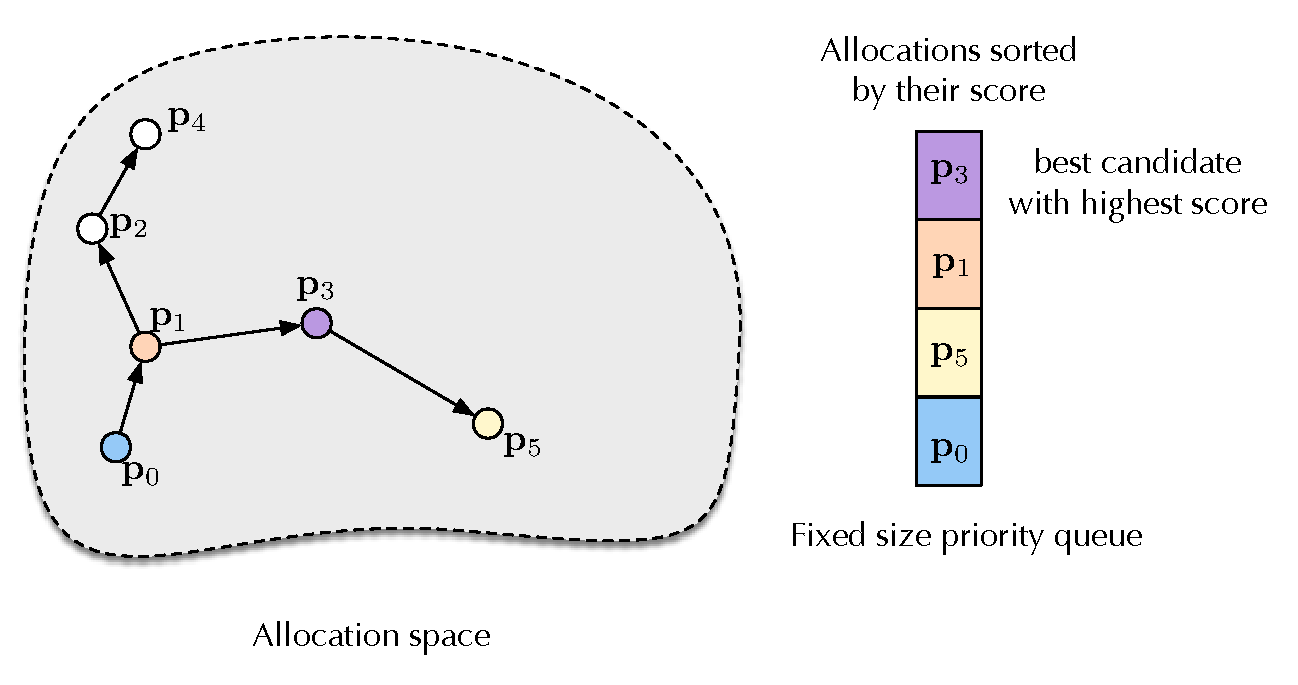
\includegraphics[width=.4\textwidth]{random-tree-figure-1}
\end{center}
\caption{Random tree with 6 sampled allocations ${\bf p}_0\dots {\bf p}_5$. Allocations are sorted in a priority queue of a a fixed size according to their score.}
\label{fig:random_tree_1}
\end{figure}

\begin{figure}[htb]
\begin{center}
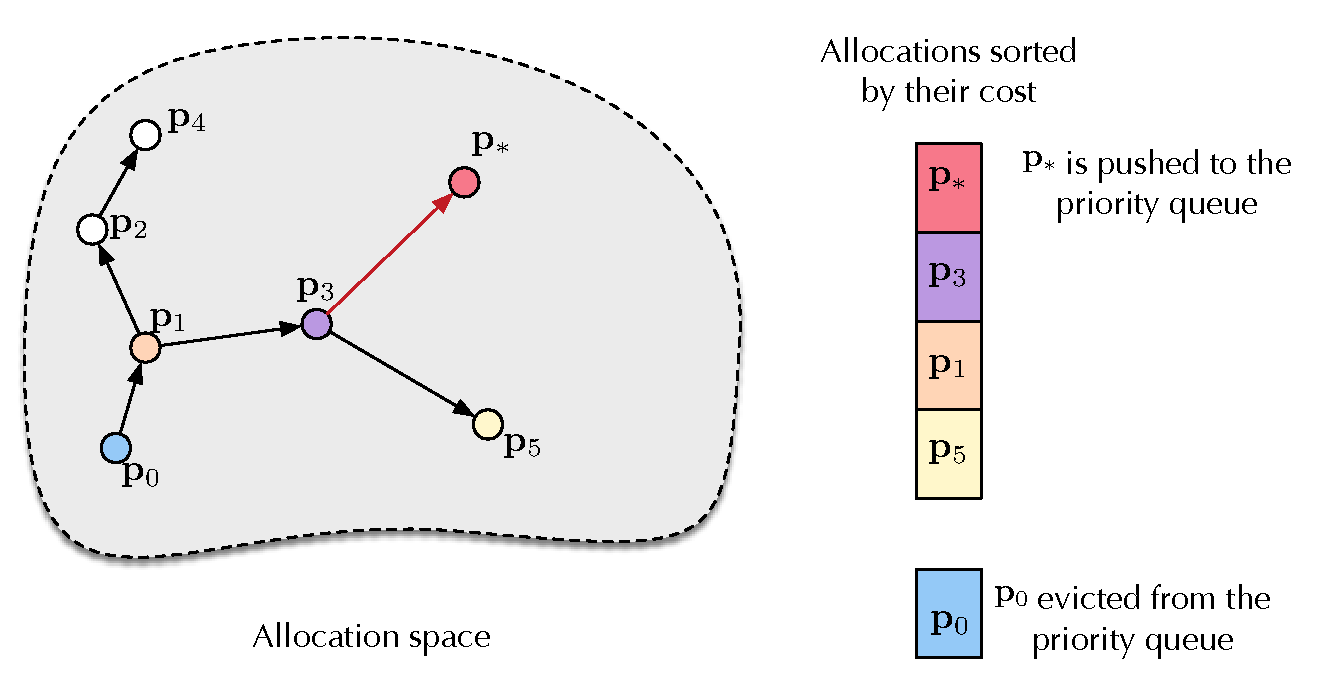
\includegraphics[width=.4\textwidth]{random-tree-figure-2}
\end{center}
\caption{After updating allocation ${\bf p}_3$, we find a new high-scoring allocation ${\bf p}_*$. Pushing ${\bf p}_*$ to the top of the queue evicts the least-scoring allocation ${\bf p}_0$. As a result, we will no longer branch the simulation from ${\bf p}_0$. }
\label{fig:random_tree_2}
\end{figure}

We utilize many heuristics to improve performance of the random tree search algorithm. We will describe these heuristics in more details.

\paragraph{Warmup phase:} Similar to other stochastic search algorithms, the runtime for random tree search depends on the choice of the initial allocation profile. In order to reduce the variance in search, the random tree starts the search by generating multiple randomized allocation as initial seeds. We emprically observed using $n$ (the number of players) iterations in the warmpup phase can substantially reduce overall runtime. In the end of warmpup phase, we sort the seeds according to their score and only keep the $b$ best seeds that we found, where $b$ is the size of the buffer.

\paragraph{Buffer size:} The buffer size $b$ has has a deep impact on how the random tree searches the allocation space. If we choose a very small buffer size, $b=1$, the random tree search becomes a greedy random walk in the space. As a result, the algorithm's performance will degrade and it can get stuck in local minimas. On the other hand,
We emprically observed setting the buffer size at a fixed size 10 yields the optimal performance.

\paragraph{Updating allocations:} At every iteration, we have to make a choice of which player's resource to update in the allocation.
The random tree algorithm updates the resources of a few of unsatisfied players in the allocation.
If we update a very few players, say 1 or 2, the algorithm converges slowly. On the other hand, if we update too many players, specially at the begining, the algorithm is unable to efficiently optimize each allocation. We updates an expected half of the players at each iteration. Furthermore, with a low probability ($5\%$), we will update a player at random (that might even be a satisfied player). These type of intentionally adding error, althought seems counter-intuitive, is shown to be very effective and practical in randomized search algorithms. 

%The random tree search algorithm work as follows.
%Initially, we generate a few random allocation as seends and compute the score of each allocation. Then we push these initial seeds into the fixed-size priority queue sorted by each allocation's score. The froniter set is the set of the $n$ highest scoring allocation that we found so far.
%At each iteration, the random tree algorithm pick an allocation from the frontier set, and changes a resource of one of the unsatisfied players. Then the random tree updates the score function and pushes back the new allocation into the frontier set.
%If the new allocation has a better score than the lowest-scoring allocation in the frontier set, we drop the least-score element from the frontier set. As a result, the frontier set always has a fixed-size.

\paragraph{Complexity Analysis:}
In order to understand the computational complexity of the random tree search algorithm, we break-down the computation at every iteration. Each iteration in the random tree search consists of three actions:
i) Picking a node from the frontier set (the priority queue) and changing the allocation,
ii) Updating the raidus and saturation of the new allocation, and
iii) Pushing back the new node back to the priority queue.
The computational complexity of the first part is $O(1)$. The most expensive part of the algorithm is updating the radius and saturation of each player, which requires running a breath-first search in the player graph. The computational complexity of running BFS is $O(n+e)$ where $n$ is the number of the players and $e$ is the number of the edges in the CSR graph. Finally, the computational complexity of inserting the new allocation back to the priority queue is $O(log b)$, where $b$ is the buffer size. Finally, we keep the priority queue sorted in order to make weighted sampling, as a result, the complexity of inserting into the priority queue is $O(b\log^2(b))$. The overal complexity of the algorithm is $O(n\times(n+e)\times b\log^2(b))$.

The random tree search algorithm is probabilistically complete \cite{Lavalle2006}. Therefore, given enought time it will always find the optimal allocation. However, there is no bound on the number of sufficient iterations for finding the optimal allocation. We emprically demonstrate the random tree requires a very few iteration to find the equilibrium points even for very large scale graphs.

\section{Experimental Results and Discussions}\label{sec:results}
We demonstrate the effectiveness and scalability of random tree search using simulation.
We implemented the random tree search algorithm in C++\footnote{Our tools and data are open-source. Our repository can be accessed at \url{github.com/ahmadyan/Capacitated-Selfish-Replication-Game}} and ran our simulation on a Macbook pro laptop equipped with Core-i7 processor and 16GB of memory.

For case-studies, we use a randomly generated Erdos-Renyi graph $G(n,p)$, where $n$ is the number of players and $p$ is the probability of existence of an edge between two player. We ensured that the graph is connected. The CSR game is for $m$ number of resources in the graph $G$. We executed the random tree search algorithm to find the optimal allocation. The random tree would terminate when the cost function reaches it's maximum at $n\times m$. For each entry point, we repeat the experiments 100 times and reported the mean number of iterations and execition time. To ensure correctness, we checked the number of unsaturated neighborhoods in the graph $G$ to be zero at termination.

Table \ref{tab:result1} shows the result of the random tree search algorithm for different games.
Our algorithm quickly found the equilibrium point in all of our experiments.

\begin{table}[]
\centering
\caption{Random tree search profile for different random graphs}
\label{tab:result1}
\begin{tabular}{lllll}
n   & p    & m  & iterations & time (s) \\
100 & 0.05 & 5  & 1453       & x        \\
100 & 0.05 & 20 & 6028       & x        \\
20  & 0.05 & 3  & 560        & x        \\
20  & 0.5  & 10 & 1045       & x
\end{tabular}
\end{table}


% two types of results:
% 1. Showing algorithm w.r.t. Number of iterations--> should be linear
% 2. Algorithm w.r.t. its runtime --> O(n^2)

\section{Conclusion}\label{sec:conclusion}
In this paper, we have studied the binary-preference capacitated selfish replication (CSR) game over general networks. We have characterized the equilibrium points of the system using a proper objective function. We leveraged this objective function and proposed a randomized algorithm based on the random tree search to find the global maximizers of this function, and hence, the NE points of the system. As an avenue for future research, one possibility is to study the dynamic version of the $CSR$ game, in the spirit of what has been discussed in \cite{fabrikant2003network}.

\bibliographystyle{IEEEtran}
\bibliography{thesisrefs}
\end{document}
